\documentclass{report}
\usepackage{fullpage,cite,amssymb,amsmath,graphicx,tabularx}
\usepackage[utf8]{inputenc}
\usepackage[nottoc]{tocbibind}

\begin{document}

\title{co2amp}
\author{Mikhail Polyanskiy}
\maketitle

\tableofcontents

\chapter{General notes}

\section{Program capabilities}
\begin{enumerate}
\item Ultrashort pulse amplification in CO$_2$ active medium
\subitem Rotational numbers up to J=60
\subitem Hot- and sequence- bands
\subitem Isotopic CO$_2$
\item Molecular dynamics
\subitem Realistic pumping
\subitem Collisional relaxation processes
\subitem Stimulated transitions
\subitem Independent consideration of active media regions at different elongation from optical axis
\item Diffraction-based beam propagation
\subitem Beam manipulation with common optical elements
\subitem Arbitrary optical configuration
\item Linear dispersion and non-linear effects in optical materials
\subitem Pulse chirping
\subitem Kerr lensing
\subitem Self-phase modulation
\item Advanced optics
\subitem Chirped-pulse amplification
\subitem Trains of pulses
\subitem Staging (program output as an input for the next stage stage)
\item User's interface
\subitem Easy parameter specification
\subitem Graphical output
\subitem Save/recall your work
\end{enumerate}

\section{Availability}
The latest version (currently 2014-xx-xx) of the co2amp program is freely available under the terms of the General Public License (GPL v.3) [] at http://www/bnl.gov/download/co2amp. The package is provided in the form of a compressed source code and as a Windows installer. The installer contains pre-compiled executables, documentation and the source-code (all found in the installation directory). User interface is built using a cross-platform library (QT by Digia []) and thus should compile under other platforms supported by QT (MacOS, Linux). Third-party components used in the package (gnuplot, 7zip) are also freely available for multiple platforms.

\section{Acknowledgements}
Viktor Platonenko provided the Mathcad code for pulse amplification in the CO$_2$ active medium that was used as a starting point of the development of the \texttt{co2amp} code; he also provided valuable input on the early stage of the work.

\chapter{Program description}

\section{Molecular dynamics}
Simulations of active medium pumping by electric discharge and vibrational relaxation are done following Karlov and Konev \cite{Karlov-1978}.

\subsection{Pumping by electric discharge}
Pumping is described by the Boltzmann equation in the following form (Karlov and Konev cite \cite{Holstein-1946} and \cite{Nighan-1970})

\begin{align}\label{eq:boltzmann}
&- \frac{1}{3} \left(\frac{E}{N}\right)^2 \frac{d}{du} \left[u \left( \sum\limits_j y_j Q_{mj}(u) \right)^{-1}\frac{df}{du} \right] \quad = \nonumber \\
&\qquad \qquad 1.09 \times 10^{ - 3}\frac{d}{du}\left[ u^2 f\sum\limits_j \frac{y_j}{M_j} Q_{mj}(u) \right]
\quad  + \quad \sum\limits_{j = 1,2} {y_j}{C_j} \frac{d}{du}(uf)
\quad  + \quad 6B y_2 \frac{d}{du}\left(uQ(u)f \right)\nonumber \\
&\qquad \qquad +\quad\sum\limits_j y_j \sum\limits_k (u + u_{jk})Q_{jk} (u + u_{jk})f(u + u_{jk}) \quad  - \quad (uf)\sum\limits_j y_j \sum\limits_k Q_{jk}(u)
\end{align}
where left part describes energy of electrons in the electric field, the first component of the sum of the right part represents energy transfer via elastic collisions between electrons and molecules, second and third components describe collisions with molecular rotation excitation, and the two last components relate to inelastic collisions with transfer of the energy $u_{jk}$ into vibrational and electronic excitation and ionization.

Electron energy $u$ is expressed in eV;

Ration of the field to the full molecular density $E/N$ is expressed in the units of $10^{-16}$ V·cm$^2$;

$y_j$ are the relative molecule concentrations ($j=1$ corresponds to CO$_2$, $j=2$ to N$_2$ and $j=3$ to He);

$M_1=44$, $M_2=28$, $M_3=4$ are the molar masses,

$C_1 = 8.2 \times 10^{-4}$ eV·Å$^2$ \cite{Hake-1967};

$C_2 = 5.06 \times 10^{-4}$ eV·Å$^2$ \cite{Frost-1962};

$B = 2.5 \times 10^{-4}$ is the N$_2$ rotational constant;

Effective crossections are expressed in Å; their numerical values in the nodes are given in the tables below (linear interpolation must be used for determining the values in intermediate points); the data and citations are reproduced from \cite{Karlov-1978}.

\begin{tabular}{|c|c||c|c||c|c||c|c|}
\hline 
$u_i$ & $Q_{m1}$ & $u_i$ & $Q_{m2}$ & $u_i$ & $Q_{m3}$ & $u_i$ & $Q$ \\ 
\hline
0    & 140  & 0     & 1.4  & 0    & 5   & 0.0015 & 0    \\
0.04 & 84   & 0.001 & 1.4  & 0.01 & 5.4 & 0.05   & 0.1  \\
0.1  & 55   & 0.002 & 1.6  & 0.1  & 5.8 & 0.25   & 0.65 \\
0.3  & 21   & 0.008 & 2    & 0.2  & 6.2 & 0.5    & 1.15 \\
0.5  & 10.8 & 0.01  & 2.2  & 1    & 6.5 & 0.8    & 2    \\
0.6  & 9.4  & 0.04  & 4    & 2    & 6.1 & 1      & 2.65 \\
1    & 5.7  & 0.08  & 6    & 7    & 5   & 1.5    & 5.6  \\
1.7  & 5    & 0.1   & 6.5  & 10   & 4.1 & 1.8    & 7.5  \\
2    & 5.1  & 0.2   & 8.8  & 20   & 3   & 1.9    & 8.2  \\
2.5  & 6    & 0.3   & 9.8  &      &     & 2      & 8.6  \\
3    & 7.7  & 0.4   & 10   &      &     & 2.15   & 8.95 \\
4.1  & 9.4  & 1     & 10   &      &     & 2.43   & 9    \\
5    & 14.5 & 1.2   & 11   &      &     & 2.6    & 8.9  \\
7.4  & 10   & 1.4   & 12.5 &      &     & 2.75   & 8.4  \\
10   & 11.7 & 1.8   & 20   &      &     & 2.9    & 7.65 \\
20   & 16   & 2     & 25   &      &     & 3.25   & 6.2  \\
27   & 16.3 & 2.5   & 30   &      &     & 3.6    & 5.1  \\
50   & 13   & 3     & 26   &      &     & 4      & 4.5  \\
     &      & 4     & 15   &      &     & 4.5    & 4.16 \\
     &      & 5     & 12   &      &     & 5      & 3.97 \\
     &      & 7     & 10   &      &     & 5.5    & 3.93 \\
     &      & 10    & 10   &      &     & 7      & 4.17 \\
     &      & 14    & 11   &      &     & 9      & 4.46 \\
     &      & 18    & 12.2 &      &     & 11     & 4.42 \\
     &      & 20    & 12   &      &     & 15     & 3.94 \\
     &      & 30    & 10   &      &     & 22     & 3.15 \\
     &      & 100   & 10   &      &     & 25     & 3.05 \\
\hline
\end{tabular}

\begin{tabular}{|c|c||c|c||c|c||c|c||c|c|}
\hline 
$u_i$ & $Q_{11}$ & $u_i$ & $Q_{12}$ & $u_i$ & $Q_{13}$ & $u_i$ & $Q_{14}$ & $u_i$ & $Q_{15}$ \\
\hline 
0.083 & 0    & 0.167 & 0    & 0.252 & 0    & 2.37 & 0    & 2.37 & 0    \\
0.085 & 0.36 & 0.2   & 0.54 & 2.7   & 0.25 & 3    & 0.26 & 3    & 0.17 \\
0.09  & 1.04 & 0.25  & 0.82 & 3     & 0.4  & 3.5  & 0.52 & 3.65 & 0.33 \\
0.1   & 1.6  & 0.3   & 0.82 & 3.3   & 0.6  & 4    & 0.5  & 3.8  & 0.31 \\
0.12  & 1.84 & 0.5   & 0.68 & 3.6   & 0.65 & 4.5  & 0.22 & 4    & 0.21 \\
0.14  & 2.12 & 0.7   & 0.56 & 4.5   & 0.23 & 4.6  & 0.1  & 4.3  & 0.1  \\
0.16  & 2.16 & 1     & 0.47 & 4.6   & 0.1  & 5    & 0    & 5    & 0    \\
0.2   & 2.08 & 1.4   & 0.45 & 5     & 0    &      &      &      &      \\
0.3   & 1.76 & 2     & 0.55 &       &      &      &      &      &      \\
0.4   & 1.52 & 3     & 1.15 &       &      &      &      &      &      \\
0.5   & 1.28 & 3.9   & 1.83 &       &      &      &      &      &      \\
0.6   & 1.08 & 4.5   & 1.4  &       &      &      &      &      &      \\
0.8   & 0.8  & 5     & 0.4  &       &      &      &      &      &      \\
1     & 0.58 & 6     & 0.28 &       &      &      &      &      &      \\
1.2   & 0.48 & 10    & 0.2  &       &      &      &      &      &      \\
1.6   & 0.34 & 20    & 0.1  &       &      &      &      &      &      \\
1.8   & 0.35 &       &      &       &      &      &      &      &      \\
2     & 0.4  &       &      &       &      &      &      &      &      \\ 
2.5   & 0.64 &       &      &       &      &      &      &      &      \\ 
3     & 1.04 &       &      &       &      &      &      &      &      \\ 
3.7   & 1.4  &       &      &       &      &      &      &      &      \\ 
4     & 1.36 &       &      &       &      &      &      &      &      \\ 
4.2   & 1.2  &       &      &       &      &      &      &      &      \\ 
4.5   & 0.92 &       &      &       &      &      &      &      &      \\ 
5     & 0.53 &       &      &       &      &      &      &      &      \\ 
6     & 0.4  &       &      &       &      &      &      &      &      \\ 
8     & 0.36 &       &      &       &      &      &      &      &      \\ 
9     & 0.28 &       &      &       &      &      &      &      &      \\ 
10    & 0.16 &       &      &       &      &      &      &      &      \\ 
10.1  & 0    &       &      &       &      &      &      &      &      \\
\multicolumn{2}{|c||}{$u_{11}=0.083$ eV} &
\multicolumn{2}{c||}{$u_{12}=0.167$ eV} &
\multicolumn{2}{c||}{$u_{13}=0.252$ eV} &
\multicolumn{2}{c||}{$u_{14}=0.339$ eV} &
\multicolumn{2}{c|}{$u_{15}=0.422$ eV}\\
\hline
\hline 
$u_i$ & $Q_{16}$ & $u_i$ & $Q_{17}$ & $u_i$ & $Q_{18}$ & $u_i$ & $Q_{19}$ & $u_i$ & $Q_{1,10}$ \\                                                                             
\hline
2.5  & 0     & 0.29 & 0    & 7    & 0     & 10.5 & 0    & 13.8 & 0    \\
3    & 0.19  & 0.3  & 0.44 & 8    & 0.5   & 11.5 & 0.56 & 15   & 0.1  \\
3.6  & 0.245 & 0.35 & 0.65 & 8.4  & 0.6   & 14   & 0.8  & 16   & 0.13 \\
4    & 0.21  & 0.4  & 0.73 & 9    & 0.46  & 20   & 1.2  & 17   & 0.17 \\
5.07 & 0     & 0.5  & 0.84 & 10   & 0.175 & 30   & 2    & 30   & 1.55 \\
     &       & 0.8  & 1    & 10.5 & 0     & 50   & 4    & 40   & 2.1  \\
     &       & 1    & 1    &      &       &      &      &      &      \\
     &       & 2    & 0.78 &      &       &      &      &      &      \\
     &       & 6    & 0.37 &      &       &      &      &      &      \\
     &       & 10   & 0.25 &      &       &      &      &      &      \\
     &       & 50   & 0    &      &       &      &      &      &      \\
\multicolumn{2}{|c||}{$u_{16}=2.5$ eV} &
\multicolumn{2}{c||}{$u_{17}=0.29$ eV} &
\multicolumn{2}{c||}{$u_{18}=7$ eV} &
\multicolumn{2}{c||}{$u_{19}=10.5$ eV} &
\multicolumn{2}{c|}{$u_{1,10}=13.8$ eV}\\
\hline 
\end{tabular}


\begin{tabular}{|c|c||c|c||c|c||c|c||c|c|}
\hline 
$u_i$ & $Q_{21}$ & $u_i$ & $Q_{22}$ & $u_i$ & $Q_{23}$ & $u_i$ & $Q_{24}$ & $u_i$ & $Q_{25}$ \\
\hline 
0.29 & 0      & 1.83  & 0     & 1.9  & 0     & 2.05 & 0     & 2.1  & 0     \\
0.5  & 0.0052 & 1.9   & 0.208 & 2    & 0.416 & 2.1  & 0.416 & 2.15 & 0.208 \\
0.8  & 0.0083 & 2     & 1.46  & 2.1  & 1.33  & 2.2  & 1.16  & 2.2  & 0.541 \\
1    & 0.0104 & 2.05  & 2.29  & 2.2  & 1.87  & 2.26 & 1.58  & 2.3  & 0.915 \\
1.2  & 0.0166 & 2.1   & 1.66  & 2.3  & 1.25  & 2.55 & 0     & 2.46 & 1.12  \\
1.3  & 0.0728 & 2.2   & 0.79  & 2.36 & 0.208 & 2.75 & 0.832 & 2.5  & 1.12  \\
1.4  & 0.135  & 2.35  & 0.208 & 2.42 & 0     & 2.77 & 0     & 2.6  & 0.208 \\
1.6  & 0.25   & 2.45  & 1.98  & 2.5  & 0.499 & 3    & 0.208 & 2.62 & 0     \\
1.8  & 0.52   & 2.5   & 1.78  & 2.61 & 0.915 & 3.05 & 0.208 & 2.68 & 0     \\
1.9  & 0.832  & 2.62  & 0.208 & 2.7  & 0.624 & 3.25 & 0     & 2.8  & 0.416 \\
2    & 3.02   & 2.75  & 1.04  & 2.75 & 0.208 &      &       & 2.9  & 0.75  \\
2.05 & 3.12   & 2.95  & 1.66  & 2.8  & 0     &      &       & 3    & 0     \\
2.1  & 2.08   & 3.05  & 0.624 & 2.92 & 0.416 &      &       & 3.2  & 0.25  \\
2.15 & 1.25   & 3.2   & 0.208 & 3    & 0.208 &      &       & 3.3  & 0.125 \\
2.2  & 0.832  & 3.4   & 0.208 & 3.25 & 0.208 &      &       & 3.35 & 0     \\
2.3  & 2.9    & 4     & 0     & 3.31 & 0     &      &       &      &       \\
2.45 & 1.04   &       &       &      &       &      &       &      &       \\
2.53 & 1.25   &       &       &      &       &      &       &      &       \\ 
2.6  & 1.75   &       &       &      &       &      &       &      &       \\ 
2.62 & 2.08   &       &       &      &       &      &       &      &       \\ 
2.68 & 1.73   &       &       &      &       &      &       &      &       \\ 
2.73 & 0.416  &       &       &      &       &      &       &      &       \\ 
2.85 & 0.32   &       &       &      &       &      &       &      &       \\ 
2.92 & 0.416  &       &       &      &       &      &       &      &       \\ 
3.12 & 0.728  &       &       &      &       &      &       &      &       \\ 
3.3  & 0.52   &       &       &      &       &      &       &      &       \\ 
4    & 0      &       &       &      &       &      &       &      &       \\ 
\multicolumn{2}{|c||}{$u_{21}=0.29$ eV} &
\multicolumn{2}{c||}{$u_{22}=0.58$ eV} &
\multicolumn{2}{c||}{$u_{23}=0.87$ eV} &
\multicolumn{2}{c||}{$u_{24}=1.16$ eV} &
\multicolumn{2}{c|}{$u_{25}=1.45$ eV}\\
\hline
\hline 
$u_i$ & $Q_{26}$ & $u_i$ & $Q_{27}$ & $u_i$ & $Q_{28}$ & $u_i$ & $Q_{29}$ & $u_i$ & $Q_{2,10}$ \\                                                                             
\hline
2.3  & 0      & 2.4   & 0     & 2.6   & 0     & 5    & 0    & 6.8  & 0     \\
2.4  & 0.75   & 2.5   & 0.208 & 2.7   & 0.208 & 5.9  & 0.41 & 7.1  & 0.57  \\
2.5  & 1.04   & 2.75  & 0.75  & 2.9   & 0.29  & 6.1  & 0.41 & 8.1  & 0.57  \\
2.55 & 1.12   & 3     & 0     & 3     & 0.208 & 7    & 0.07 & 8.6  & 0.25  \\
2.6  & 1.04   & 3.2   & 0.166 & 3.1   & 0     & 9    & 0    & 9.5  & 0.12  \\
2.65 & 0.624  & 3.3   & 0.146 & 3.2   & 0     &      &      & 20.7 & 0     \\
2.7  & 0.416  & 3.4   & 0     & 3.3   & 1.04  &      &      &      &       \\
2.8  & 0.208  &       &       & 3.4   & 0     &      &      &      &       \\
2.9  & 0.125  &       &       &       &       &      &      &      &       \\
3    & 2.5    &       &       &       &       &      &      &      &       \\
3.1  & 0.166  &       &       &       &       &      &      &      &       \\
3.2  & 0      &       &       &       &       &      &      &      &       \\
\multicolumn{2}{|c||}{$u_{26}=1.74$ eV} &
\multicolumn{2}{c||}{$u_{27}=2.03$ eV} &
\multicolumn{2}{c||}{$u_{28}=2.32$ eV} &
\multicolumn{2}{c||}{$u_{29}=5$ eV} &
\multicolumn{2}{c|}{$u_{2,10}=6.8$ eV}\\
\hline
\hline 
$u_i$ & $Q_{2,11}$ & $u_i$ & $Q_{2,12}$ & $u_i$ & $Q_{2,13}$ & $u_i$ & $Q_{2,14}$ & $u_i$ & $Q_{2,15}$ \\                                                                             
\hline
8.4  & 0      & 11.25 & 0     & 12.5  & 0     & 14   & 0    & 15.6 & 0     \\
8.7  & 0.42   & 13.8  & 0.41  & 13    & 0.4   & 14.3 & 1.7  & 18   & 0.1   \\
9.1  & 0.42   & 14    & 1     & 13.6  & 0.4   & 14.8 & 1.7  & 20   & 0.21  \\
10   & 0.3    & 14.7  & 1     & 14    & 0.16  & 15.6 & 0.2  & 50   & 2.52  \\
20.7 & 0      & 15    & 0.25  & 20.7  & 0     & 20.6 & 0.2  & 100  & 2.52  \\
     &        & 65    & 0     &       &       & 25.4 & 2.8  &      &       \\
     &        &       &       &       &       & 100  & 2.8  &      &       \\
\multicolumn{2}{|c||}{$u_{2,11}=8.4$ eV} &
\multicolumn{2}{c||}{$u_{2,12}=11.25$ eV} &
\multicolumn{2}{c||}{$u_{2,13}=12.5$ eV} &
\multicolumn{2}{c||}{$u_{2,14}=14$ eV} &
\multicolumn{2}{c|}{$u_{2,15}=15.6$ eV}\\
\hline 
\end{tabular} 

The following notation for cross-sections is used:

$Q_{m1}$ - Transport cross-section of {CO$_2$} \cite{Lowke-1973};

$Q_{m2}$ - Transport cross-section of {N$_2$} \cite{Frost-1962};

$Q_{m3}$ - Transport cross-section of He \cite{Lowke-1973};

$Q$ - Cross-section of resonant excitation of {N$_2$} rotation  \cite{Oksyuk-1966,Chandra-1973};

$Q_{11}$ - Cross-section of the process $(000)\rightarrow(01^10)$  \cite{Lowke-1973};

$Q_{12}$ - Cross-section of the process $(000)\rightarrow(100+020)$  \cite{Lowke-1973};

$Q_{13}...Q_{16}$ - Cross-sections of resonant processes around 3.8 eV  \cite{Lowke-1973};

$Q_{17}$ - Cross-section of the process $(000)\rightarrow(001)$  \cite{Lowke-1973};

$Q_{18}...Q_{1,10}$ - Cross-sections of electronic excitation and ionization of {CO$_2$}  \cite{Hake-1967};

$Q_{21}...Q_{28}$ - Cross-sections of the process {N$_2$}$(v=0)\rightarrow${N$_2$}$(v=1...8)$ \cite{Phelps-1968,Schulz-1962,Engelhardt-1964};

$Q_{29}...Q_{2,15}$ - Cross-sections of electronic excitation and ionization of {N$_2$} \cite{Engelhardt-1964}.  

Equation \ref{eq:boltzmann} is solved numerically using the tridiagonal matrix algorithm.
Rate constant $omega_{jk}$ and electron drift speeds $v_d$ are defined as:

\begin{equation}\label{eq:omega_jk}
\omega _{jk}\left[\frac{\rm{cm}^3}{\text{s}} \right] = 5.93 \times 10^{-9}\int\limits_0^\infty u Q_{jk}(u)f(u)du
\end{equation}
     
\begin{equation}\label{eq:v_d}
v_d \left[ \frac{\text{cm}}{\text{s}} \right] =  - 5.93 \times 10^7 \left( \frac{1}{3}\frac{E}{N} \right)\frac{df}{du} \int\limits_0^\infty u \left( \sum\limits_j y_j Q_{mj}(u) \right)^{-1} du
\end{equation}

Fraction of electron energy transmitted via inelastic processes is defined as:

\begin{equation}\label{eq:z_jk}
z_{jk} = 10^6 \frac{y_j u_{jk} \omega _{jk}} {\left( \frac{E}{N} \right) v_d}   
\end{equation}

Fraction of electron energy transmitted to translations and rotations are:

\begin{equation}\label{eq:z_t}
z_t = 5.93 \times 10^7 \frac{\int\limits_0^\infty u^2 \left( \sum\limits_j \frac{y_j}{M_j} Q_{mj}(u) \right)f(u)du} {\left( \frac{E}{N} \right) v_d}
\end{equation}

\begin{equation}\label{eq:z_r}
z_r = 5.93 \times 10^7 \frac{\sum\limits_{j=1,2} y_j C_j \int\limits_0^\infty uf(u)du + 6 y_2 B \int\limits_0^\infty u Q(u) f(u) du} {\left( \frac{E}{N} \right) v_d} 
\end{equation}

Then, for 4-temperature model we get:

$q_2 = \sum\limits_{k=1}^6 z_{1k}$ - fraction of energy transferred to {CO$_2$} symmetric stretch ($\nu_1$) and bending ($\nu_2$) modes;

$q_3 = z_{17}$ - fraction of energy transferred to {CO$_2$} asymmetric stretch mode ($\nu_3$);

$q_4 = \sum\limits_{k=1}^8 z_{2k}$ - fraction of energy transferred to {N$_2$} vibrations;

$q_T = z_t + z_r$ - fraction of energy transferred to translation and rotation;

$q_{ei} = \sum\limits_{k=9}^{15} z_{2k}  + \sum\limits_{k=8}^{10} z_{1k}$ - fraction of energy spent on electronic levels excitation and ionization.


\subsection{Pumping and vibrational relaxation dynamics}
3-temperature model is used for describing vibrational dynamics of the laser system

$T_2$ – vibrational temperature of $\nu_1$ and $\nu_2$ vibrations of{CO$_2$};

$T_3$ – vibrational temperature of the $\nu_3$ vibration of {CO$_2$};

$T_4$ – vibrational temperature of {N$_2$}.

Vibrational temperatures are related to average number of quanta $e_x$ in the corresponding vibrations as:

\begin{align}\label{eq:e}
&{e_2} = \frac{2}{\exp(960/{T_2})-1}  \nonumber\\
&{e_3} = \frac{1}{\exp(3380/{T_3})-1} \\
&{e_4} = \frac{1}{\exp(3350/{T_4})-1} \nonumber
\end{align}
("2" in the first equation is due to 2-fold degeneracy of the bend vibration levels).

Pumping/relaxation dynamics is described by the following equations \cite{Karlov-1978}

\begin{align}\label{eq:dedt}
&\frac{d e_4}{dt} = p_{e4} - r_a (e_4 - e_3)\nonumber\\
&\frac{d e_3}{dt} = p_{e3} + r_c(e_4 - e_3) - r_3 f_3\\
&\frac{d e_2}{dt} = f_2 \left( p_{e2} + 3 r_3 f_3 - r_2 (e_2 - e_{2T}) \right)\nonumber
\end{align}

where

\begin{align*}
&p_{e4} = 0.8\times 10^{-3} \frac{q_4}{n y_2} W(t);\quad p_{e3} = 0.8\times 10^{-3}\frac{q_3}{n y_1} W(t);\quad p_{e2} = 2.8\times 10^{-3}\frac{q_2}{n y_1} W(t);\\
&f_2 = \frac{2(1+e_2)^2}{2+6e_2+3{e_2}^2};\quad f_3 = e_3(1+e_2/2)^3 - (1+e_3)(e_2/2)^3 \exp(- 500/T);\\
&r_a = kny_1;\quad r_c = kny_2;\quad r_2 = k_2n;\quad r_3 = k_3n;\\
&k_2 = \sum\limits_{i=1}^3 y_i k_{2i};\quad k_3 = \sum\limits_{i=1}^3 y_i k_{3i};\\
&n = 273 \frac{p[\text{bar}]}{T_0[\text{K}]},
\end{align*}
where $W(t)$ is measured in {kW/cm$^3$} , $p_e$ - in {$\mu$s}, and constants $k$ are calculated using the following expressions \cite{Biryukov-1974,Taylor-1969}:

\begin{align*}
&k = 240 / T^{1/2};\\
&k_{31} = A(t)\exp(4.138 + 7.945x - 631.24x^2 + 2239x^3);\\
&k_{32} = A(t)\exp(-1.863 + 213.3x - 2796.2x^2 + 9001.9x^3);\\
&k_{33} = A(t)\exp(-3.276 + 291.4x - 3831.8x^2 + 12688x^3);\\
&k_{21} = 1.16 \times 10^3 \exp(-59.3x);\\
&k_{22} = 8.55 \times 10^2 \exp(-69x);\\
&k_{22} = 1.3 \times 10^3 \exp(-40.6x),
\end{align*}
where $x=T^{-1/3}$, $A(t)=(T/273)(1+e_{2T}/2)^{-3}$, and temperature is expressed in K.


Finally, the gas temperature dynamics is described by the Equation \ref{eq:dTdt}

\begin{equation}\label{eq:dTdt}
\frac{dT}{dt} = \frac{y_1}{C_V}(500r_3f_3 + 960r_2(e_2-e_{2T})) + 2.7\frac{W(t)q_T}{nC_V},
\end{equation}
where $C_V = 2.5(y_1+y_2) + 1.5y_3$.


\section{Amplification}

Amplification is simulated using the equations from Volkin’s paper \cite{Volkin-1979}

\begin{align}\label{eq:amplification}
&\frac{1}{c}\frac{\partial \varepsilon}{\partial t} + \frac{\partial \varepsilon}{\partial z} =  - \sum\limits_J {\rho _J},\nonumber\\
&\frac{\partial \rho _J}{\partial t} + \left(i(\omega _c-\omega _{0J}) + \frac{1}{T_2} \right)\rho _J =  - \frac{\sigma _J n_J \varepsilon}{2T_2},\\
&\frac{\partial n_J}{\partial t} + \frac{n_J-n_J^0}{\tau _R} = 4(\rho _J \varepsilon^* + c.c.), \nonumber
\end{align}
where $\varepsilon(z,t)$ is the complex field envelope, $\omega _c$ the carrier frequency, $\omega_{0J}$ the frequency in the line center and $\sigma_J$ the stimulated emission (or absorption) cross-section in the line center:

\begin{equation*}
{\sigma _J}[\text{m}^2] = \frac{(\lambda _J[\text{m}])^2 A_J[\text{s}^{-1}]}{4} \times \frac{T_2[\text{s}]}{\pi},
\end{equation*}
where the first term defines the integral cross-section $\sigma_0$ of the rotational line \cite{Hilborn-2002} and the second term is the maximum of the normalized Lorentzian profile of a line with linewidth $\Delta\omega _{FWHM}=2\pi\Delta\nu=2/T_2$,

\begin{equation*}
n_J^0 = z(J)(N^U-N^L),
\end{equation*}
where $z(J)$ is the Boltzmann distribution:

\begin{align*}
&z(J) = 2\frac{hB}{kT}(2J+1)\exp \left(-\frac{hB}{kT}J(J+1)\right)&626, 636, 828, 838\\
&z(J) = \frac{hB}{kT}(2J+1)\exp \left(-\frac{hB}{kT}J(J+1)\right)&628, 638
\end{align*}

$h = 6.62606957\times 10^{-34}$ J·s

$k = 1.3806488\times 10^{-23}$ J/K

$B$: [s$^{-1}$]

$T$: [K]

Field amplitude is related to the intensity as follows:

\begin{equation}\label{eq:I}
I[\text{W/m}^2] = 2 h[\text{J·s}] \nu _c[\text{s}^{-1}] \varepsilon ^2
\end{equation}

Additional equations:

\begin{align}\label{eq:dNdt}
&\frac{d}{dt}N^U = 2\sum\limits_J (\rho _J\varepsilon _J^* + c.c.) ,\nonumber\\
&\frac{d}{dt}N^{L10} =  -2\sum\limits_{J10} (\rho _J\varepsilon _J^* + c.c.),\\
&\frac{d}{dt}N^{L9} =  -2\sum\limits_{J9} (\rho _J\varepsilon _J^* + c.c.)\nonumber
\end{align}

Relaxation times are defined from the following equations:

\begin{equation}\label{eq:T2}
T_2[\text{s}] = \frac{10^{- 6}}{\pi \times 7.61 \times 750 \times (P_{CO2}+0.733P_{N2}+0.64P_{He})}
\end{equation}

\begin{equation}\label{eq:tauR}
\tau _R[\text{s}] = \frac{10^{-7}}{750 \times (P_{CO2}+1.2P_{N2}+0.6P_{He})}
\end{equation}

$P$ is measured in Bar.

\begin{equation*}
\Delta\nu _{FWHM} = \frac{1}{\pi T_2}
\end{equation*}

Useful relations for Lorentzian distribution:

\begin{equation*}
\Delta\nu _{HWHM} = \frac{1}{2\pi T_2};\quad \Delta\omega _{HWHM} = \frac{1}{T_2}
\end{equation*}


\section{Propagation}

Beam propagation between layout elements is calculated using Huygens-Fresnel integration at each time-step of the pulse time-frame. In the general case, the field in a given position $(x',y')$ of the output plane is calculated by integrating contributions from each point $(x,y)$ of the input plane taken into account the phase delay.

\begin{equation*}
E(x', y') = \int_x\int_y E(x,y) \frac{e^{ikR}}{i\lambda R} dx dy,
\end{equation*}
where $k$ is the wave number, $\lambda$ the wavelength, and $R$ is the distance between points $(x,y)$ in and $(x',y')$ in the output plane: $R=\sqrt{(x-x')^2+(y-y')^2+\Delta z^2}$. $\Delta z$ is the distance between the centers of the input and the output planes.

In the case of radially symmetric beam used in our model, calculations can be considerably accelerated by taken into account that the field is the same in all points at equal distance from the beam axis. In this case integration can be done by summing the contributions of concentric rings in the input plane as shown in the Fig. \ref{fig:Huygens-Fresnel}.

\begin{figure}[ht]
\centering
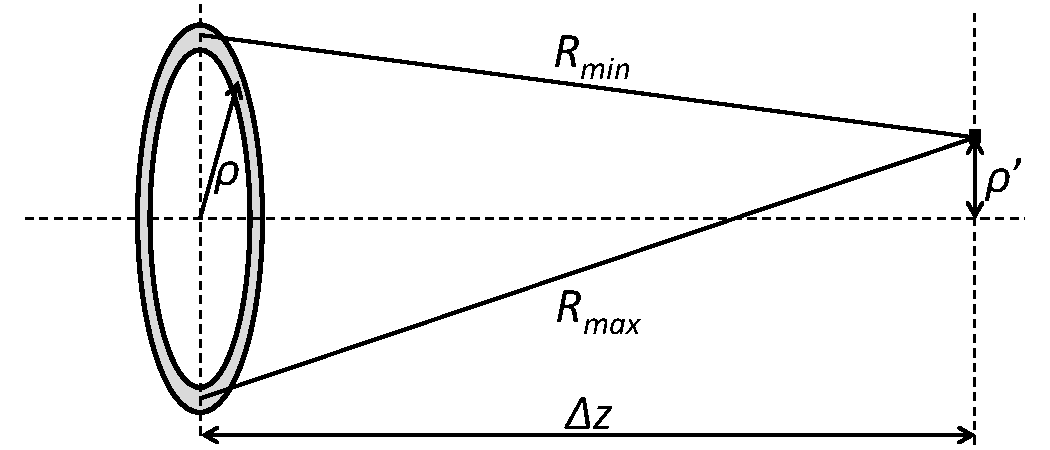
\includegraphics[width=120mm]{images/huygens-fresnel}
\caption{Huygens-Fresnel integration in the axial-symmetric system: Contribution of a field from a concentric ring in the input plane to a field in a point in the output plane.}\label{fig:Huygens-Fresnel}
\end{figure}

The field in a given point with radial coordinate $\rho'$ in the output plane is then calculated as

\begin{equation}
E(\rho') = \int_{\rho}E(\rho)\frac{e^{-ikR}}{i\lambda R} J_0(k\Delta R/2) dS
\end{equation}
where $dS = \pi(\rho+d\rho/2)^2-\pi(\rho-d\rho/2)^2$ is the area of the ring, $R=(R_{max}+R_{min})/2$, $\Delta R=R_{max}-R_{min}$, $R_{max}=\sqrt{(\rho+\rho')^2+\Delta z^2}$, $R_{min}=\sqrt{(\rho-\rho')^2+\Delta z^2}$, and $J_0$ is the Bessel function.


\section{Optical elements}
Optical elements change the electric field as described by the following formulas. In these formulas $E$ is the field in the input of the element and $E'$ - after passing through the element.

\subsection{Lens}
\begin{equation}
E'(\rho) = E(\rho) e^{2\pi i \frac{\rho^2}{2 \lambda F}},
\end{equation}
where $F$ is the focal length of the lens and $\lambda$ is the central wavelength.

\subsection{Absorber}
\begin{equation}
E'(\rho) = E(\rho) \sqrt{T},
\end{equation}
where $T$ is the transmittance.

\subsection{Mask}
\begin{align}
&E'(\rho) = 0, &\rho < R\\
&E'(\rho) = E(\rho), &\rho \geq R
\end{align}
where $R$ is the radius of the mask.


\chapter{Getting started manual}


\section{Basic concepts}
The \texttt{co2amp} code allows simulating propagation of an ultrashort pulse through an arbitrary optical system that can include CO$_2$ amplifiers. Pulse amplification and fast molecular dynamics (stimulated transitions, rotational relaxation) calculations are performed in time domain in the time-frame moving with the pulse. Processes that are much slower than the pulse duration (discharge pumping, vibrational relaxation) are modelled separately in the laboratory time-frame.
The program input parameters include initial pulse characteristics, optical configuration, active medium composition and excitation parameters (e.g. discharge profile), and number of nodes in the calculation grids for the time- (pulse time frame) and space- (radial) coordinates. Axial symmetry is assumed at all times. Optical system can include multiple amplifiers if they have same gas composition and pumping dynamics; sequential amplification in different amplifiers can be modeled using the staging option as described later.
Temporal pulse shape (averaged across the beam) and beam profile (averaged for the entire pulse duration) at every element of the optical layout are saved and can be accessed in both graphical and tabulated-numerical representation. Complete pulse/beam information (complex field in every node of the time-space calculation grid) at the output of the system can also be saved and used as an input for another system (staging).
The user interface program allows saving all inputs and outputs of the calculations as a single compressed file ('.co2' or '.co2x' extension). The difference between the two formats is that the files with extension ending with 'x' ("extended") include the complete output field record and thus are suitable for staged calculations.
Fig. \ref{fig:co2amp} shows the user interface of the \texttt{co2amp} program described in the following sections.

\begin{figure}[ht]
\centering
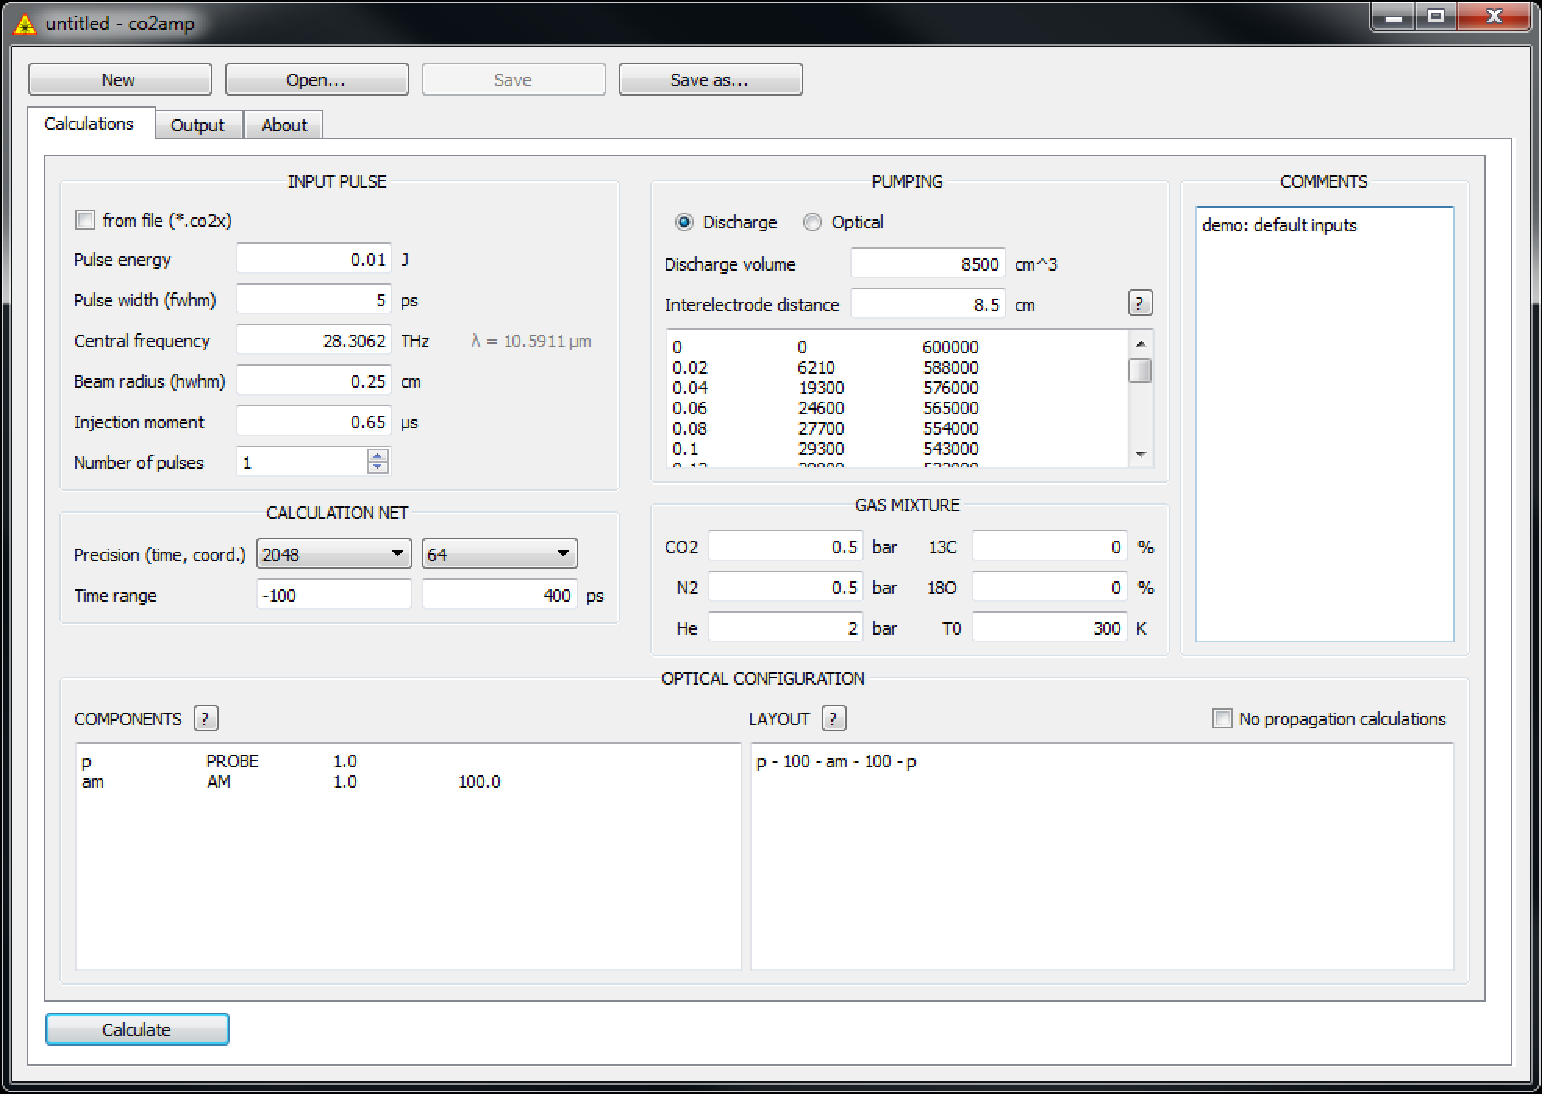
\includegraphics[width=8cm]{images/co2amp-input}
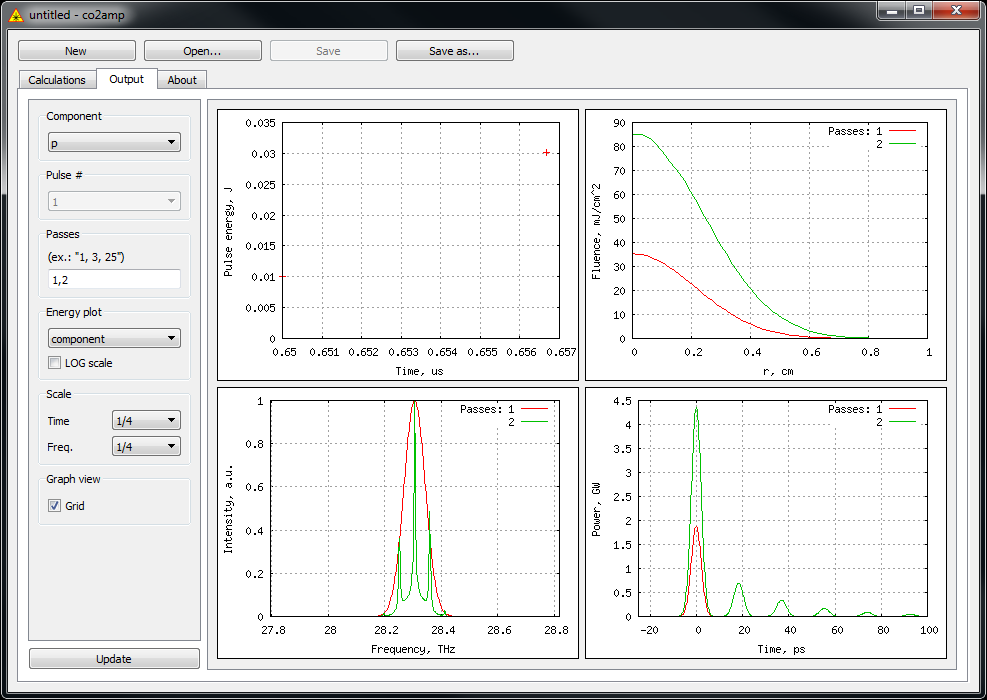
\includegraphics[width=8cm]{images/co2amp-output}
\caption{\texttt{co2amp} user interface: Input- (left) and output- (right) tabs.}\label{fig:co2amp}
\end{figure}


\section{Input pulse and calculation grid}
Unless the output of another simulation is used as an input (staged calculations), both temporal shape of the input pulse and the input beam profile are assumed to be Gaussian; and the pulse is assumed to be transform-limited (no initial chirping). Pulse energy, duration, central frequency, and beam radius are entered in the corresponding fields in the input tab. "Injection moment" parameter specifies the time-delay between the beginning of the pumping of the active medium and pulse injection into the optical system. It is also possible to simulate amplification of a train of identical and equidistant pulses; number of pulses in the train and time-delay between them must be specified in this case.
Number of nodes in the calculation grid has to be specified for the radial coordinate and for the fast time-frame associated with the pulse (time-frame for the slow processes uses a fixed 1-ns step and does not require a user input). Number of nodes is always a power of two that allows utilization of fast Fourier transform (FFT) algorithms. Calculations with a larger number of nodes are usually more accurate but, on the other hand, take longer and require more computer memory (both calculation time and required memory are roughly proportional to the product of the number of  nodes in the time- and space- grids). This is therefore recommended to start from running the simulation with a smaller number of nodes and then repeat it several times, each time with a denser grid. Absence of considerable change in the program output with increase of the number of nodes will indicate that the grid density is sufficient.
Limits of the pulse time-frame ("time range") specify the time interval considered in the calculations. Initially, the pulse is centered at $t=0$ and it tends to shift to the longer delays upon amplification due to the limited medium response time and spectrum modulation. Thus, optimum time range is usually asymmetric with a short negative and a longer positive part. Time-step $\Delta t=(t_{max}-t_{min})/(n_0-1)$, where $t_{max}$ and $t_{min}$ define the time range and $n_0$ is the number of nodes in the time grid, must be small enough to accurately describe the pulse profile at all stages of the propagation through the optical system. It is also important to keep in mind that time range and number of nodes in the time grid also define the range and step in the frequency domain: $\Delta\nu=1/(t_{max}-t_{min})$ and $(\nu_{max}-\nu_{min})=1/\Delta t$. This means that the time range must be long enough to provide sufficient resolution in the frequency domain and at the same time the time step must be sufficiently short to provide a bandwidth that fits the whole spectral region of interest.
Maximum radial coordinate is defined separately for every element of the optical system. This is described in the next section.
Identifying an appropriate calculation grid is very important for building an accurate model of an optical system. An effort put in this part of the simulation process will pay off by fast and reliable calculations.


\section{Optical layout and beam propagation}
The \texttt{co2amp} code uses a concept of optical surfaces similar to that employed in the ray-tracing algorithms. In this concept optical system is represented by a series of thin optical components (surfaces) each of which can alter the wave front. Between surfaces, beam propagates undisturbed. In order to specify the optical system one has to 1) describe all optical components and 2) describe the location of the components in respect to each other. In \texttt{co2amp}'s user interface program, this is done by editing text in the two dedicated fields ("Components" and "Layout"). The format of these fields is described below.

\subsection{Components}
Each optical component is described in a separate line by several tab- or space- separated entries:

\begin{itemize}
\item Entry 1 '\textit{\textbf{ID}}': An arbitrary user-defined alpha-numeric string for identifying the component;
\item Entry 2 '\textit{\textbf{Type}}': Type of the component; must be one of the types listed in the table;
\item Entry 3 '\textit{\textbf{Field}}':  Maximum radial coordinate in centimeters to be considered in the simulations;
\item Entry 4 '\textit{\textbf{Parameter 1}}' and Entry 5 '\textit{\textbf{Parameter 2}}': Meaning of these fields depend on the type of the component as summarized in the table:
\end{itemize}

\def\tabularxcolumn#1{m{#1}}
\begin{tabularx}{\textwidth}{|l|X|X|X|}
\hline 
\textit{\textbf{Type}} & Description & \textit{\textbf{Parameter 1}} & \textit{\textbf{Parameter 2}} \\
\hline 
&&&\\
\texttt{AM}	& Active medium	& Length [cm]	& - \\
&&&\\
\texttt{PROBE} & Passive surface, may be used as limiting aperture &	- &	-\\
&&&\\
\texttt{MASK} & Opaque circular screen & Radius [cm] & -\\
&&&\\
\texttt{ABSORBER} & Absorber & Transmittance & -\\
&&&\\
\texttt{LENS} & Ideal lens (no spherical or chromatic aberrations)& Focal length [cm]& -\\
&&&\\
\texttt{WINDOW} & Transparent flat window (zero reflection- and absorption- losses) & Window material: KCl, NaCl, ZnSe, Ge, GaAs, Diamond, or CdTe & Thickness [cm]\\

\texttt{STRETCHER} & Stretcher or compressor & Pulse chirping [ps/THz] (positive for red-chirp) & -\\
\hline
\end{tabularx}\\


The following example defines several 2.5-cm diameter components: A probe surface, two 120-cm-long amplifier sections, a 5-cm-thick NaCl window and an absorber for modelling 4\% reflection losses:

\bigskip
\begin{tabular}{lllll}
\texttt{p}   & \texttt{PROBE}    & \texttt{1.25} &               &           \\
\texttt{am1} & \texttt{AM}       & \texttt{1.25} & \texttt{120}  &           \\
\texttt{am2} & \texttt{AM}       & \texttt{1.25} & \texttt{120}  &           \\
\texttt{win} & \texttt{WINDOW}   & \texttt{1.25} & \texttt{NaCl} & \texttt{5}\\
\texttt{abs} & \texttt{ABSORBER} & \texttt{1.25} & \texttt{0.96} &
\end{tabular}

\subsection{Layout}
Optical configuration is specified as a sequence of the components identified by their \textit{\textbf{ID}}’s. All components are separated by non-negative distances expressed in centimeters. Components and distances must be separated by spaces, tabs, new-line symbols or dashes. The following is an example of an optical configuration that uses the components defined in the previews example:

\bigskip
\texttt{p-0-abs-0-win-0-abs-100-am1-200-am2-100-abs-0-win-0-abs-0-p }
\bigskip

This example defines the configuration shown in the Fig. \ref{fig:optical-configuration-1}.

\begin{figure}[ht]
\centering
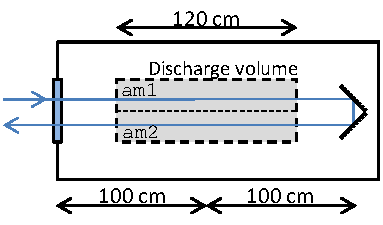
\includegraphics{images/optical-configuration-1}
\caption{Example optical configuration.}\label{fig:optical-configuration-1}
\end{figure}

In this example beam propagates twice through the same amplifier. However, we consider this configuration as two identical but independent active volumes (\texttt{am1} and \texttt{am2}) because at each pass the beam interacts with a different zone of the active medium.

\subsection{Beam propagation}
When two components of an optical configuration are separated by a non-zero distance, beam propagation between them is simulated using the Huygens-Fresnel diffraction integral in the assumption of axial symmetry. Propagation is simulated separately for each moment of time from the time calculation grid.
Optical surface model assumes that components of the optical layout are infinitely thin. Propagation is calculated between the middle points of the components; for the purpose of simulating pulse interaction with a prolonged optical element, beam is assumed to be collimated inside this element. For instance, the sequence of calculations for the previews example is:

\begin{enumerate}
\item Interaction with the window (including reflection losses);
\item 100 cm propagation to the middle of the first pass through the amplifier (no amplification so far);
\item Amplification by a 120-cm amplifier section assuming that the beam is collimated;
\item 200 cm (100$\times$2) propagation to the middle of the second pass through the active volume;
\item Amplification by the second 120-cm amplifier section assuming that the beam is collimated;
\item 100 cm propagation to the window;
\item Interaction with the windows.
\end{enumerate}

Accuracy of the model can be improved if one divides a long amplifier into several shorter sub-sections. For instance, we can modify our example configuration as shown in the Fig. \ref{fig:optical-configuration-2}.

\begin{figure}[ht]
\centering
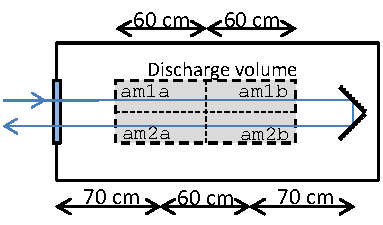
\includegraphics{images/optical-configuration-2}
\caption{Example configuration modified for improved accuracy.}\label{fig:optical-configuration-2}
\end{figure}
 
Components and Layout entries for the modified configuration are as follows:

\bigskip
Components:

\bigskip
\begin{tabular}{lllll}
\texttt{p}   & \texttt{PROBE}    & \texttt{1.25} &               &           \\
\texttt{am1a} & \texttt{AM}      & \texttt{1.25} & \texttt{60}  &           \\
\texttt{am1b} & \texttt{AM}      & \texttt{1.25} & \texttt{60}  &           \\
\texttt{am2a} & \texttt{AM}      & \texttt{1.25} & \texttt{60}  &           \\
\texttt{am2b} & \texttt{AM}      & \texttt{1.25} & \texttt{60}  &           \\
\texttt{win} & \texttt{WINDOW}   & \texttt{1.25} & \texttt{NaCl} & \texttt{5}\\
\texttt{abs} & \texttt{ABSORBER} & \texttt{1.25} & \texttt{0.96} &
\end{tabular}
\bigskip

Layout:

\bigskip
\texttt{p-0-abs-0-win-0-abs-70-am1a-60-am1b-140-am2b-60-am2a-70-abs-0-win-0-abs-0-p}
\bigskip

Population dynamics in all amplifier sections is modeled separately and thus splitting a long amplifier into shorter sections provides also a more realistic model of the active medium.


\section{Active medium and amplification}
All active medium sections used in a single simulation must have same gas composition and pumping conditions (staged simulations can be used for complex systems with two or more non-identical amplifiers).  Composition (including isotopic enrichment of carbon dioxide) and initial temperature of the active medium are specified in the "Gas Mixture" fields of the input tab of the user interface.
Pumping by electric discharge is the primary pumping scheme of the \texttt{co2amp} code. Rudimentary support for optical pumping is also included but not discussed here. For discharge pumping, geometry of the discharge volume (discharge volume and the distance between electrodes) and discharge profile (tabulated values of discharge current expressed in amperes and voltage in volts at time moments in microseconds) must be provided. Pumping dynamics calculations are done using a Boltzmann equation that takes into account elastic collisions between electrons and molecules and inelastic collisions with molecular rotational-, vibrational- and electronic- excitations and ionization. Tabulated empirical values of corresponding cross-sections as functions of electron energy are used. The Boltzmann equation is solved repeatedly in order to accurately describe the variation of pumping efficiency by the electric field varying during the discharge. 


\section{Program output}
The output of the program is given as a temporal pulse structure and its spectrum (both averaged across the beam) and beam profile (averaged on the duration of the pulse) at each element of the optical layout. The user can chose an optical component to display from the list of all the available components. In the case if the selected component is used several times in the optical configuration, it is also possible to specify which passes through the component will be displayed. Also, integral pulse energy can be provided either at every pass through a selected component or at all passes through all components of the system layout.
Output for the layout components of type \texttt{AM} (active medium) provides additional information that includes gain, discharge profile, population dynamics, and the dynamics of pumping energy distribution (fractions of discharge energy going into excitation of laser levels and excitation of molecular translations and ionization).
Right-mouse-click on a figure allows the user to copy either the graphics or the numerical data for future use.

                          
\bibliographystyle{unsrt}
\bibliography{co2amp}
                          
\end{document}            